\newpage
\section{実験結果}
選定したシナリオ 28 例中,24例の自律移動を確認した.
以下は1例として Scenario35 を走行時の実験の様子を\figref{fig:exp_path}に示す.

\begin{figure*}[htbp]
    \begin{tabular}{ccc}
        \begin{minipage}[t]{0.5\textwidth}
            \centering
            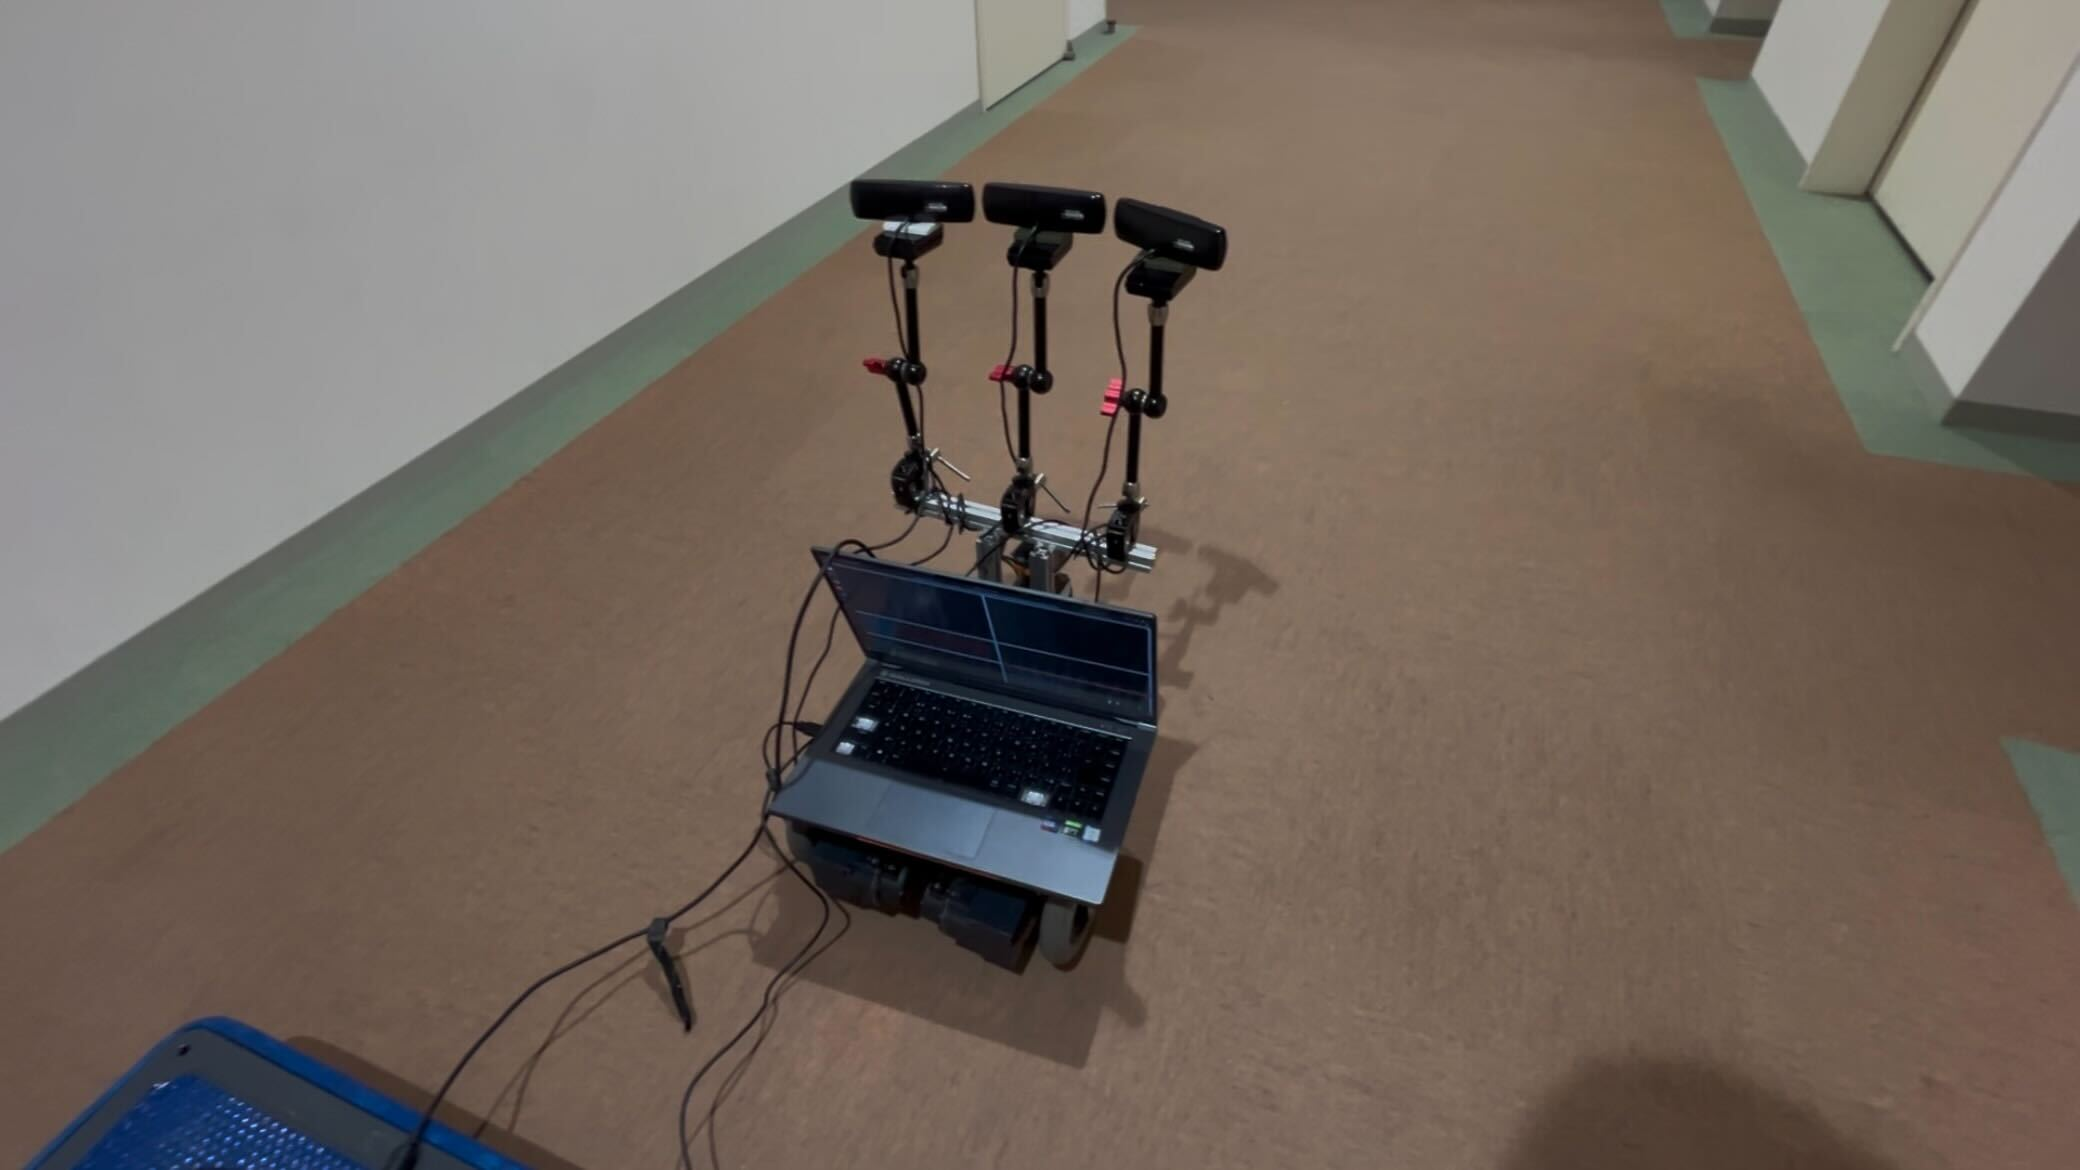
\includegraphics[keepaspectratio, width=55mm]{images/png/ishiguro/exp_0.png}
            \subcaption{突き当たりまで直進}
        \end{minipage} &
        \begin{minipage}[t]{0.5\textwidth}
            \centering
            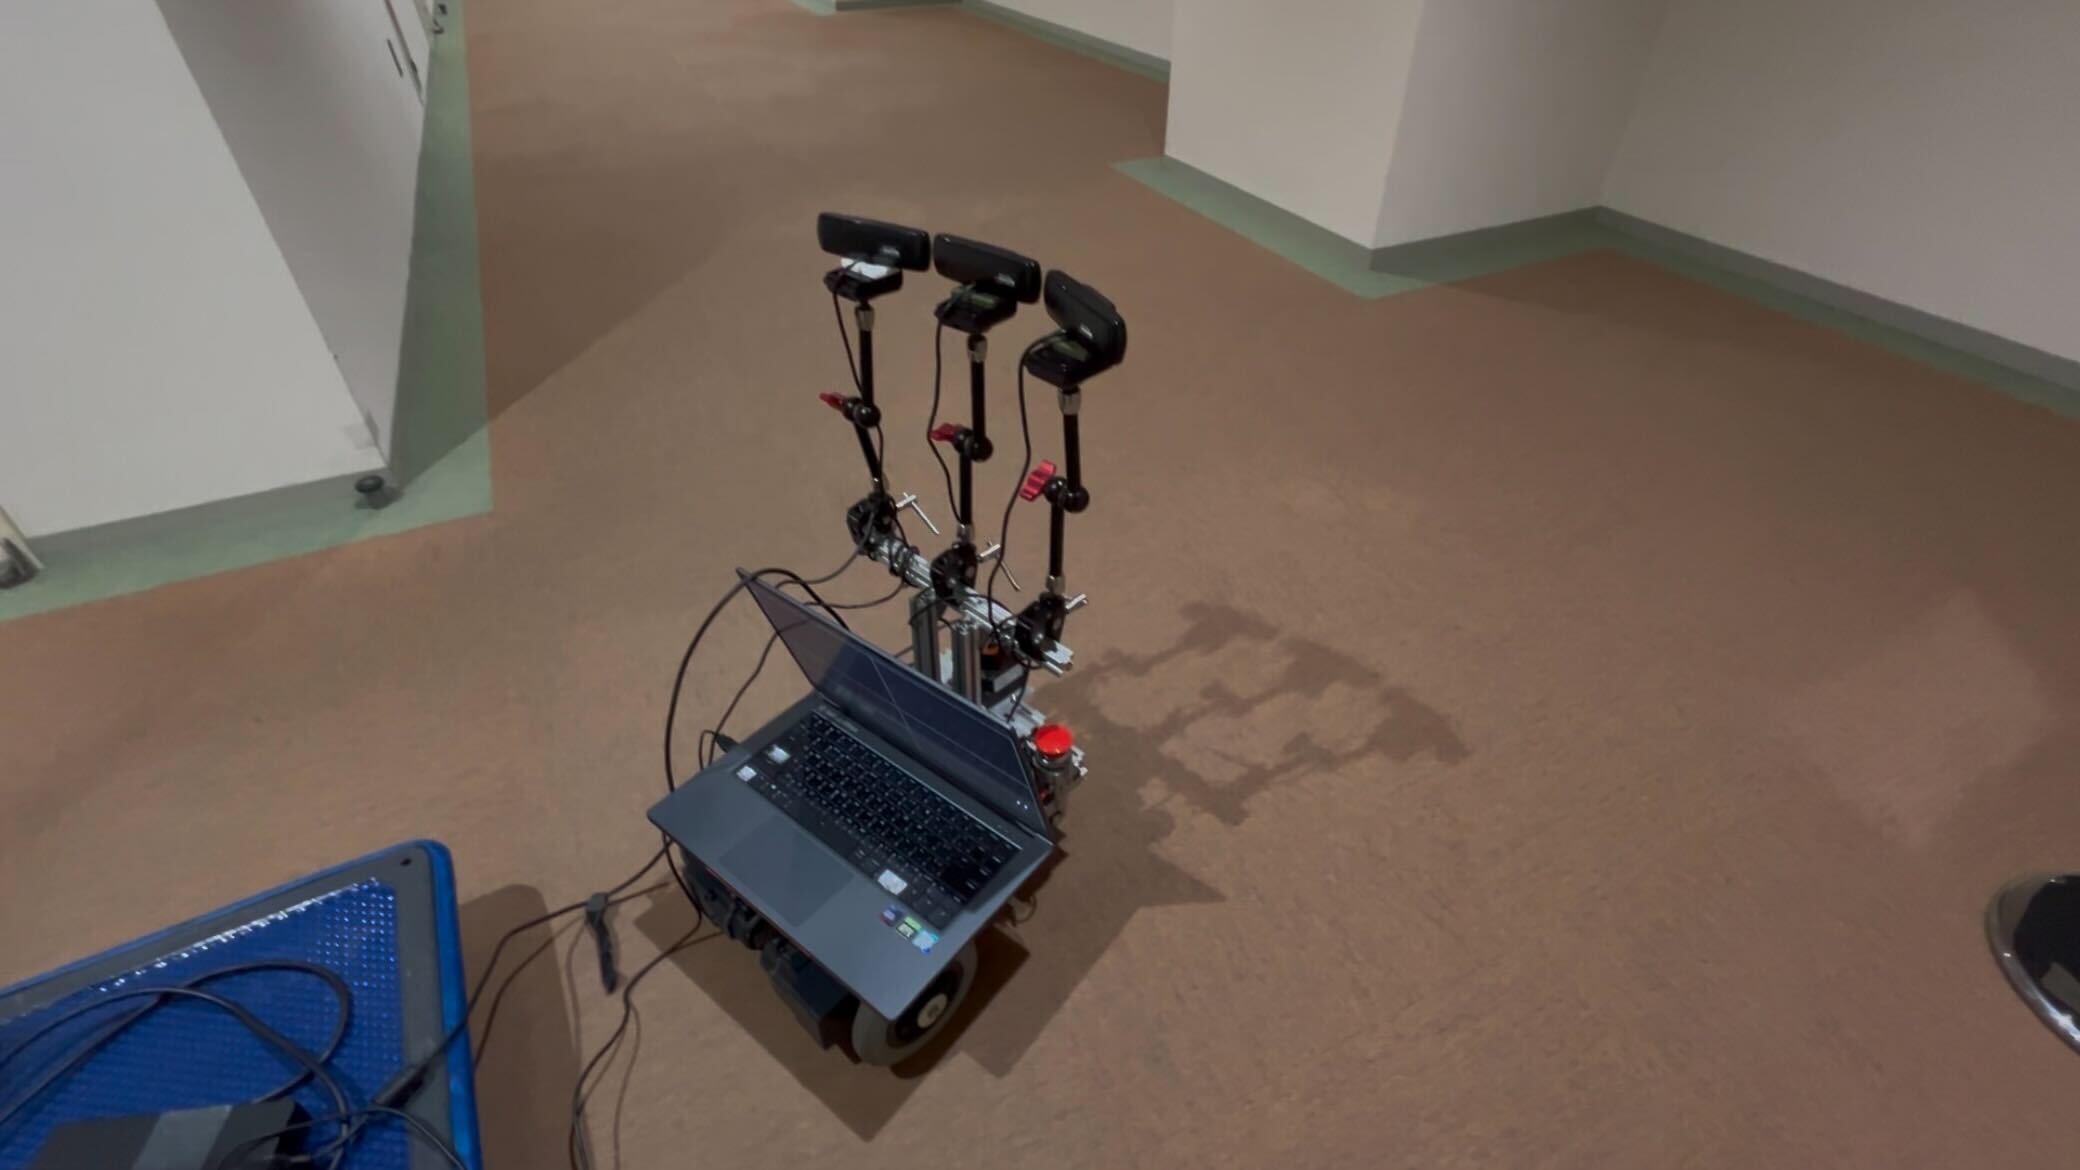
\includegraphics[keepaspectratio, width=55mm]{images/png/ishiguro/exp_1.png}
            \subcaption{左折}
        \end{minipage} \\
        \begin{minipage}[t]{0.5\textwidth}
            \centering
            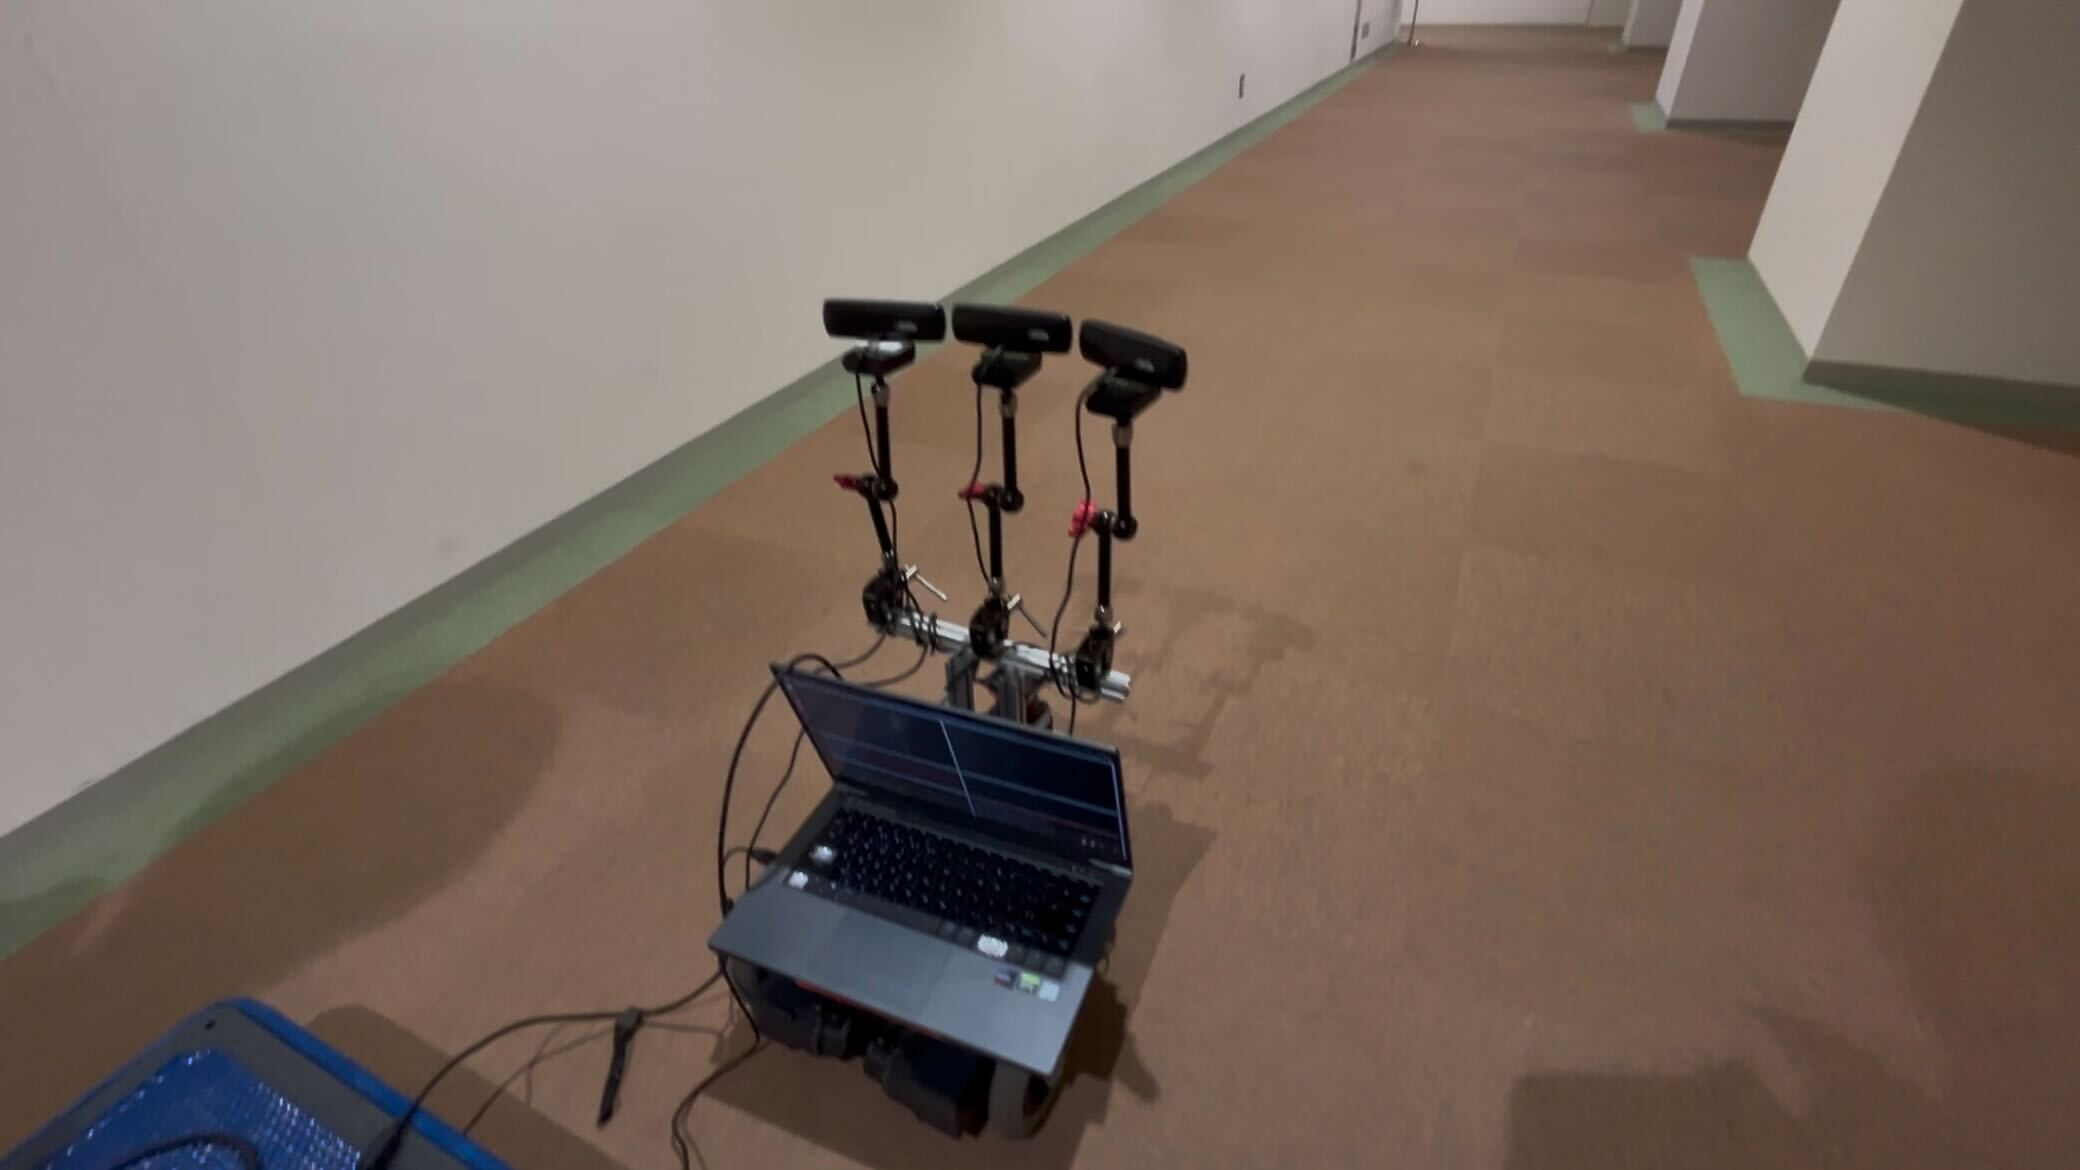
\includegraphics[keepaspectratio, width=55mm]{images/png/ishiguro/exp_2.png}
            \subcaption{突き当たりまで直進}
        \end{minipage} &
        \begin{minipage}[t]{0.5\textwidth}
            \centering
            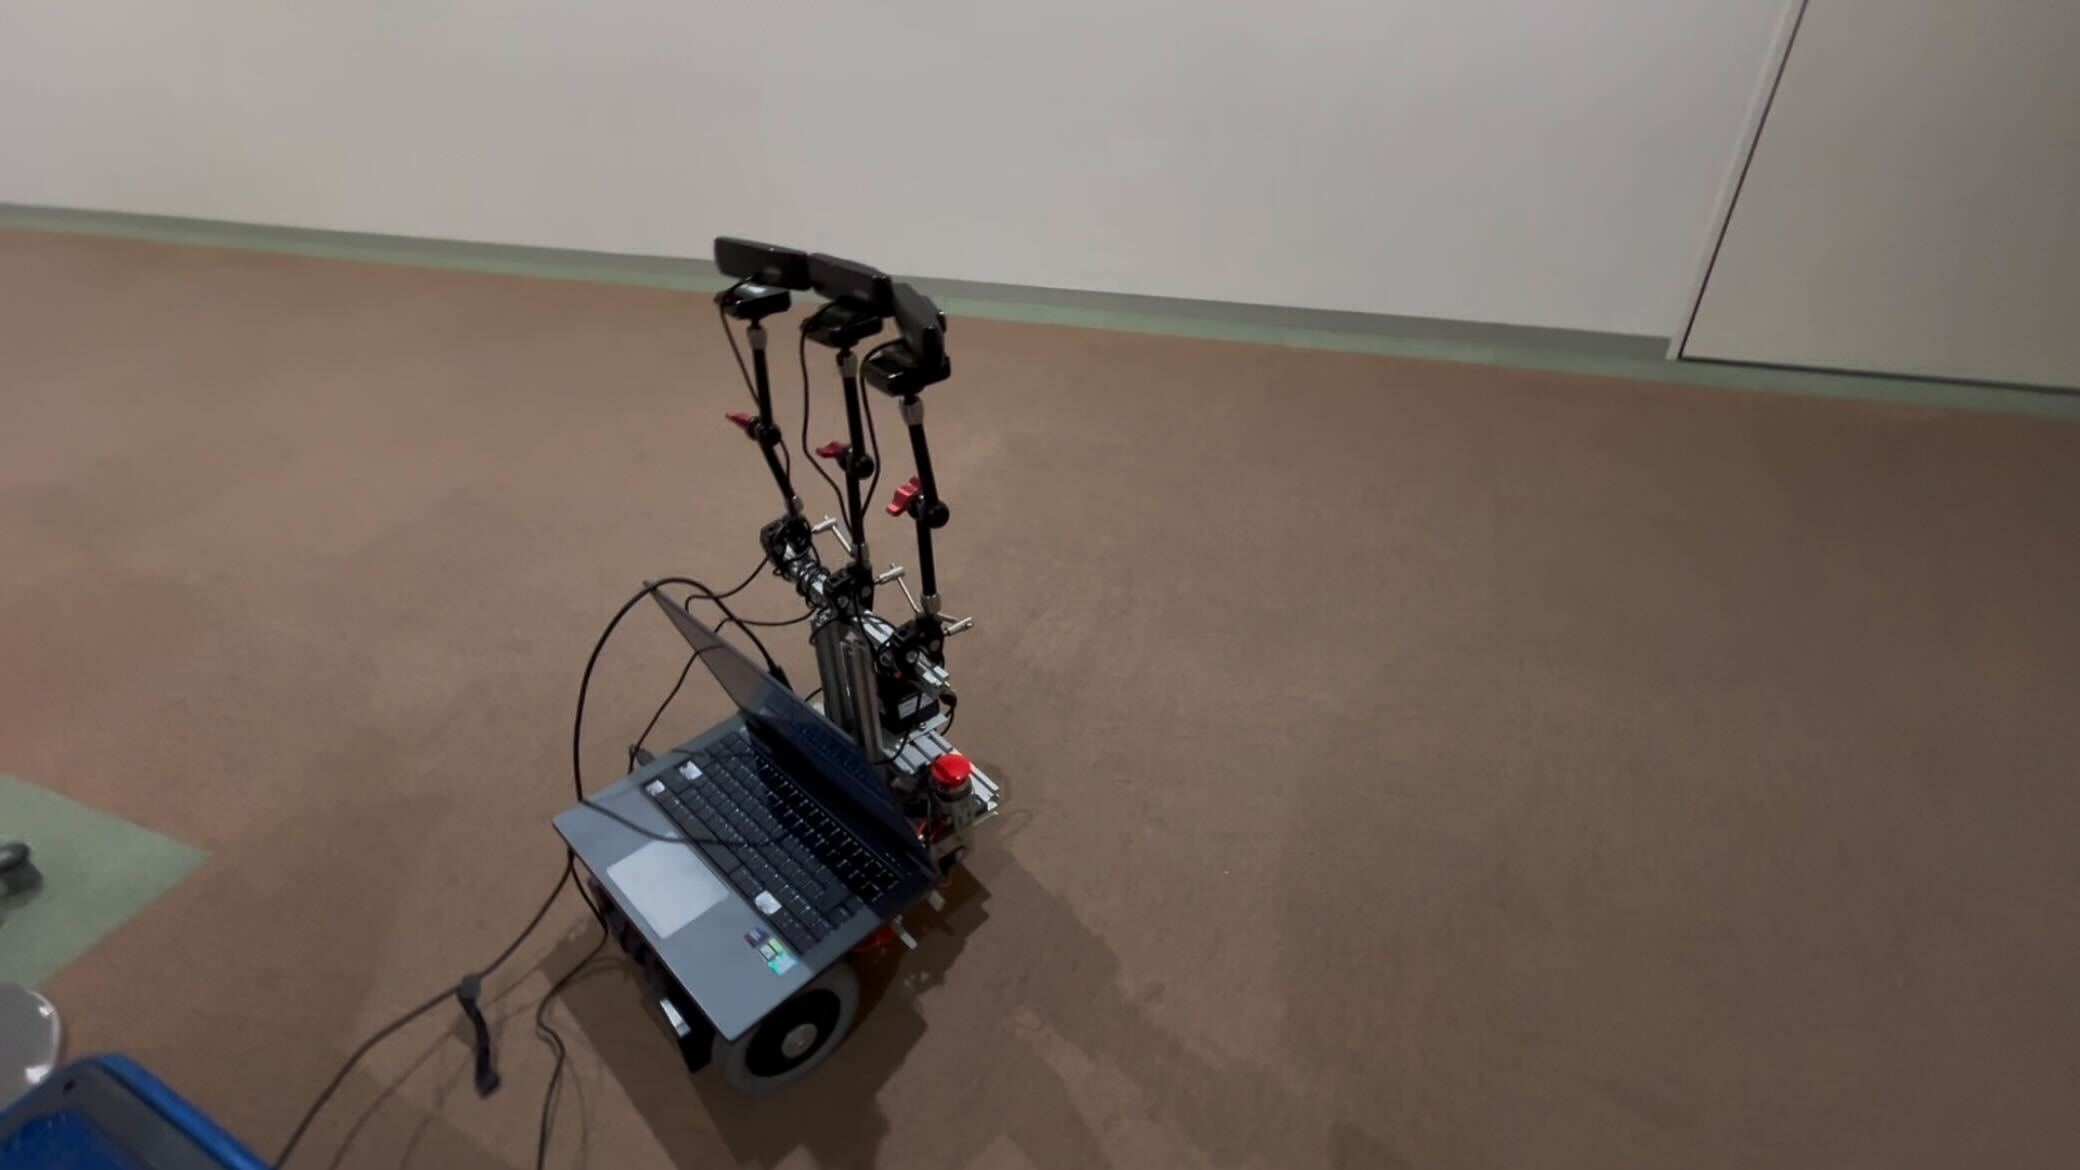
\includegraphics[keepaspectratio, width=55mm]{images/png/ishiguro/exp_3.png}
            \subcaption{右折}
        \end{minipage} \\
        \begin{minipage}[t]{0.5\textwidth}
            \centering
            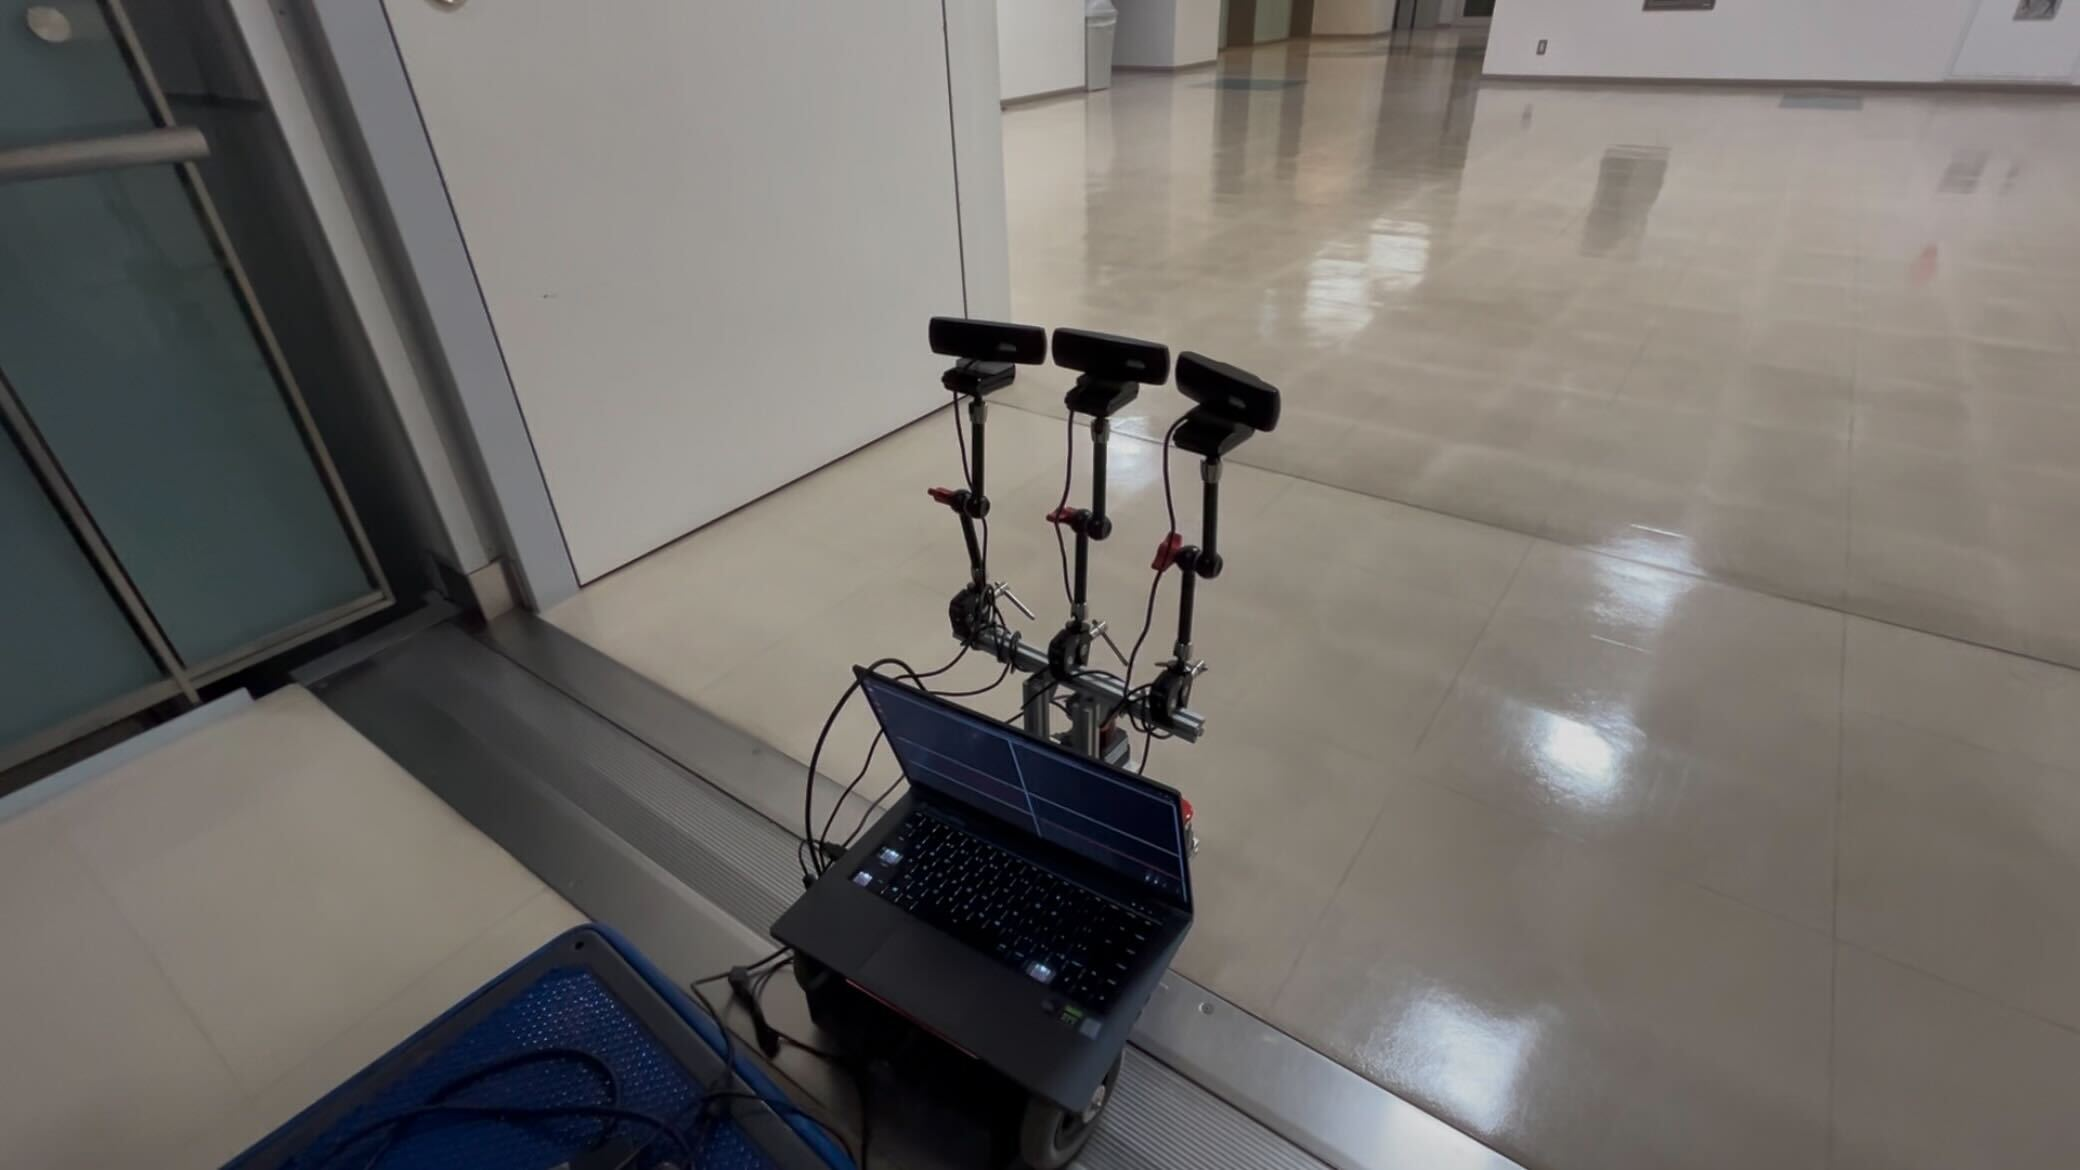
\includegraphics[keepaspectratio, width=55mm]{images/png/ishiguro/exp_4.png}
            \subcaption{突き当たりまで直進}
        \end{minipage} &
        \begin{minipage}[t]{0.5\textwidth}
            \centering
            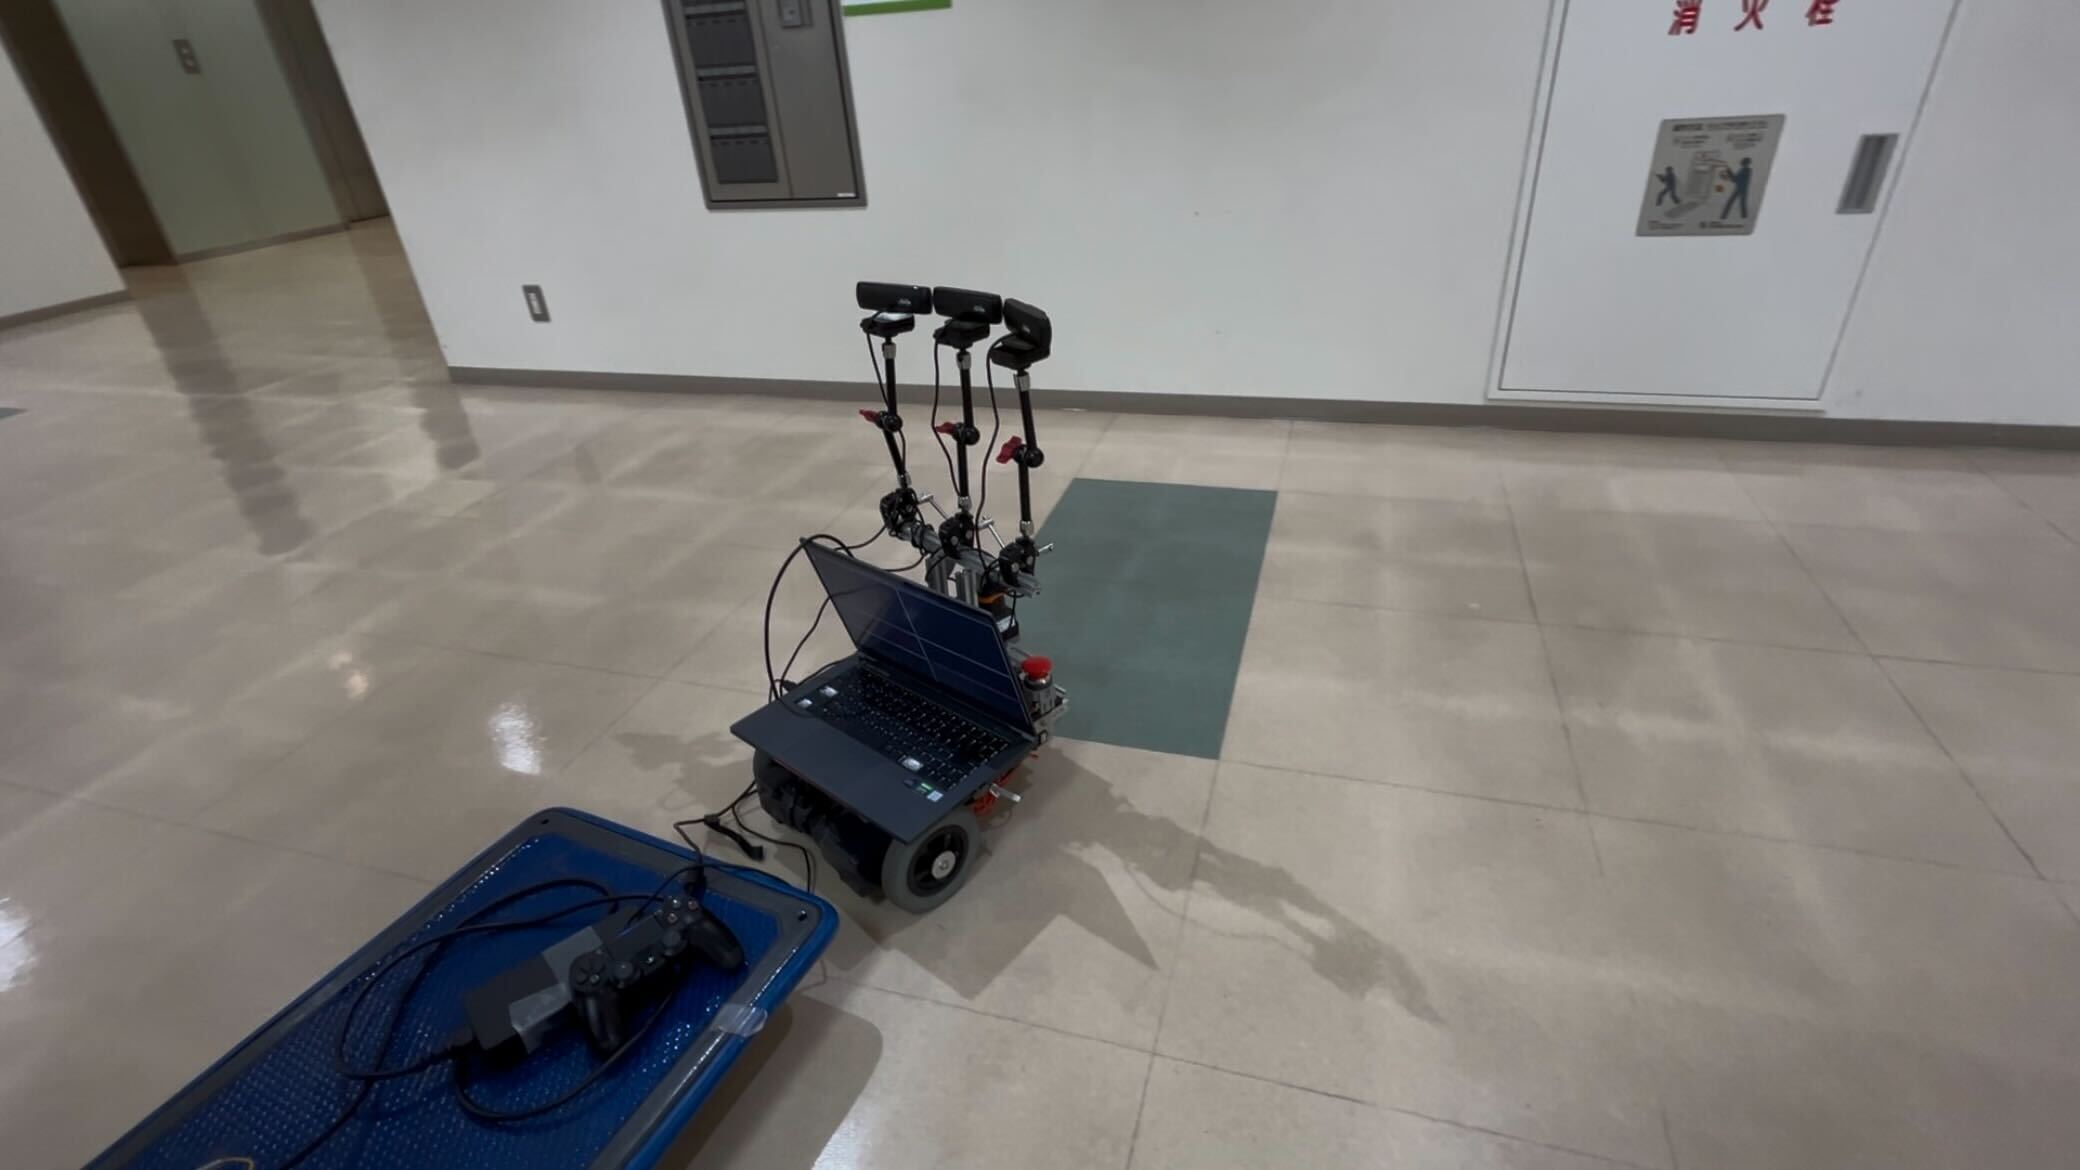
\includegraphics[keepaspectratio, width=55mm]{images/png/ishiguro/exp_5.png}
            \subcaption{右折}
        \end{minipage} \\
        \begin{minipage}[t]{0.5\textwidth}
            \centering
            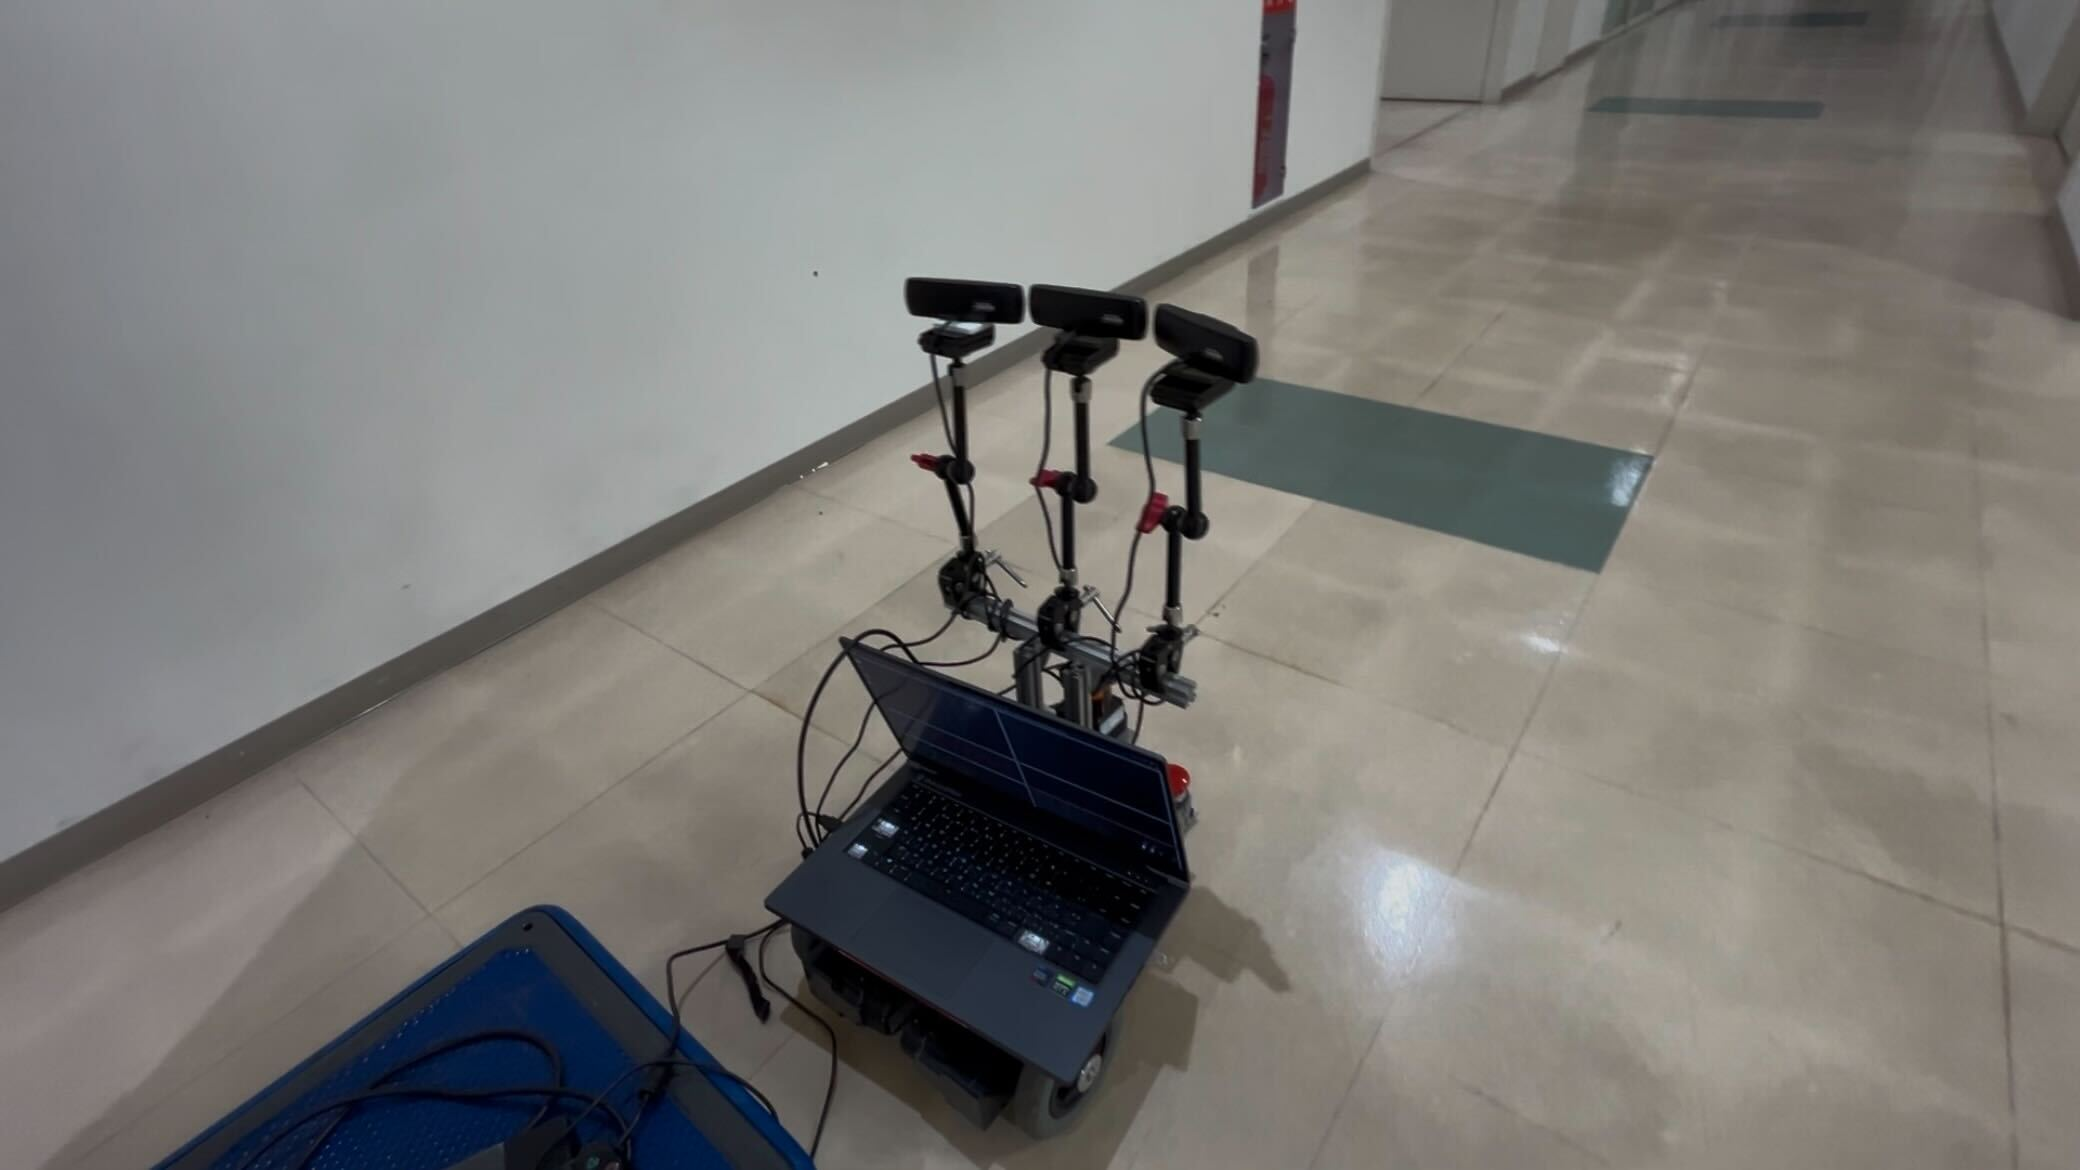
\includegraphics[keepaspectratio, width=55mm]{images/png/ishiguro/exp_6.png}
            \subcaption{次の角まで直進}
        \end{minipage} &
        \begin{minipage}[t]{0.5\textwidth}
            \centering
            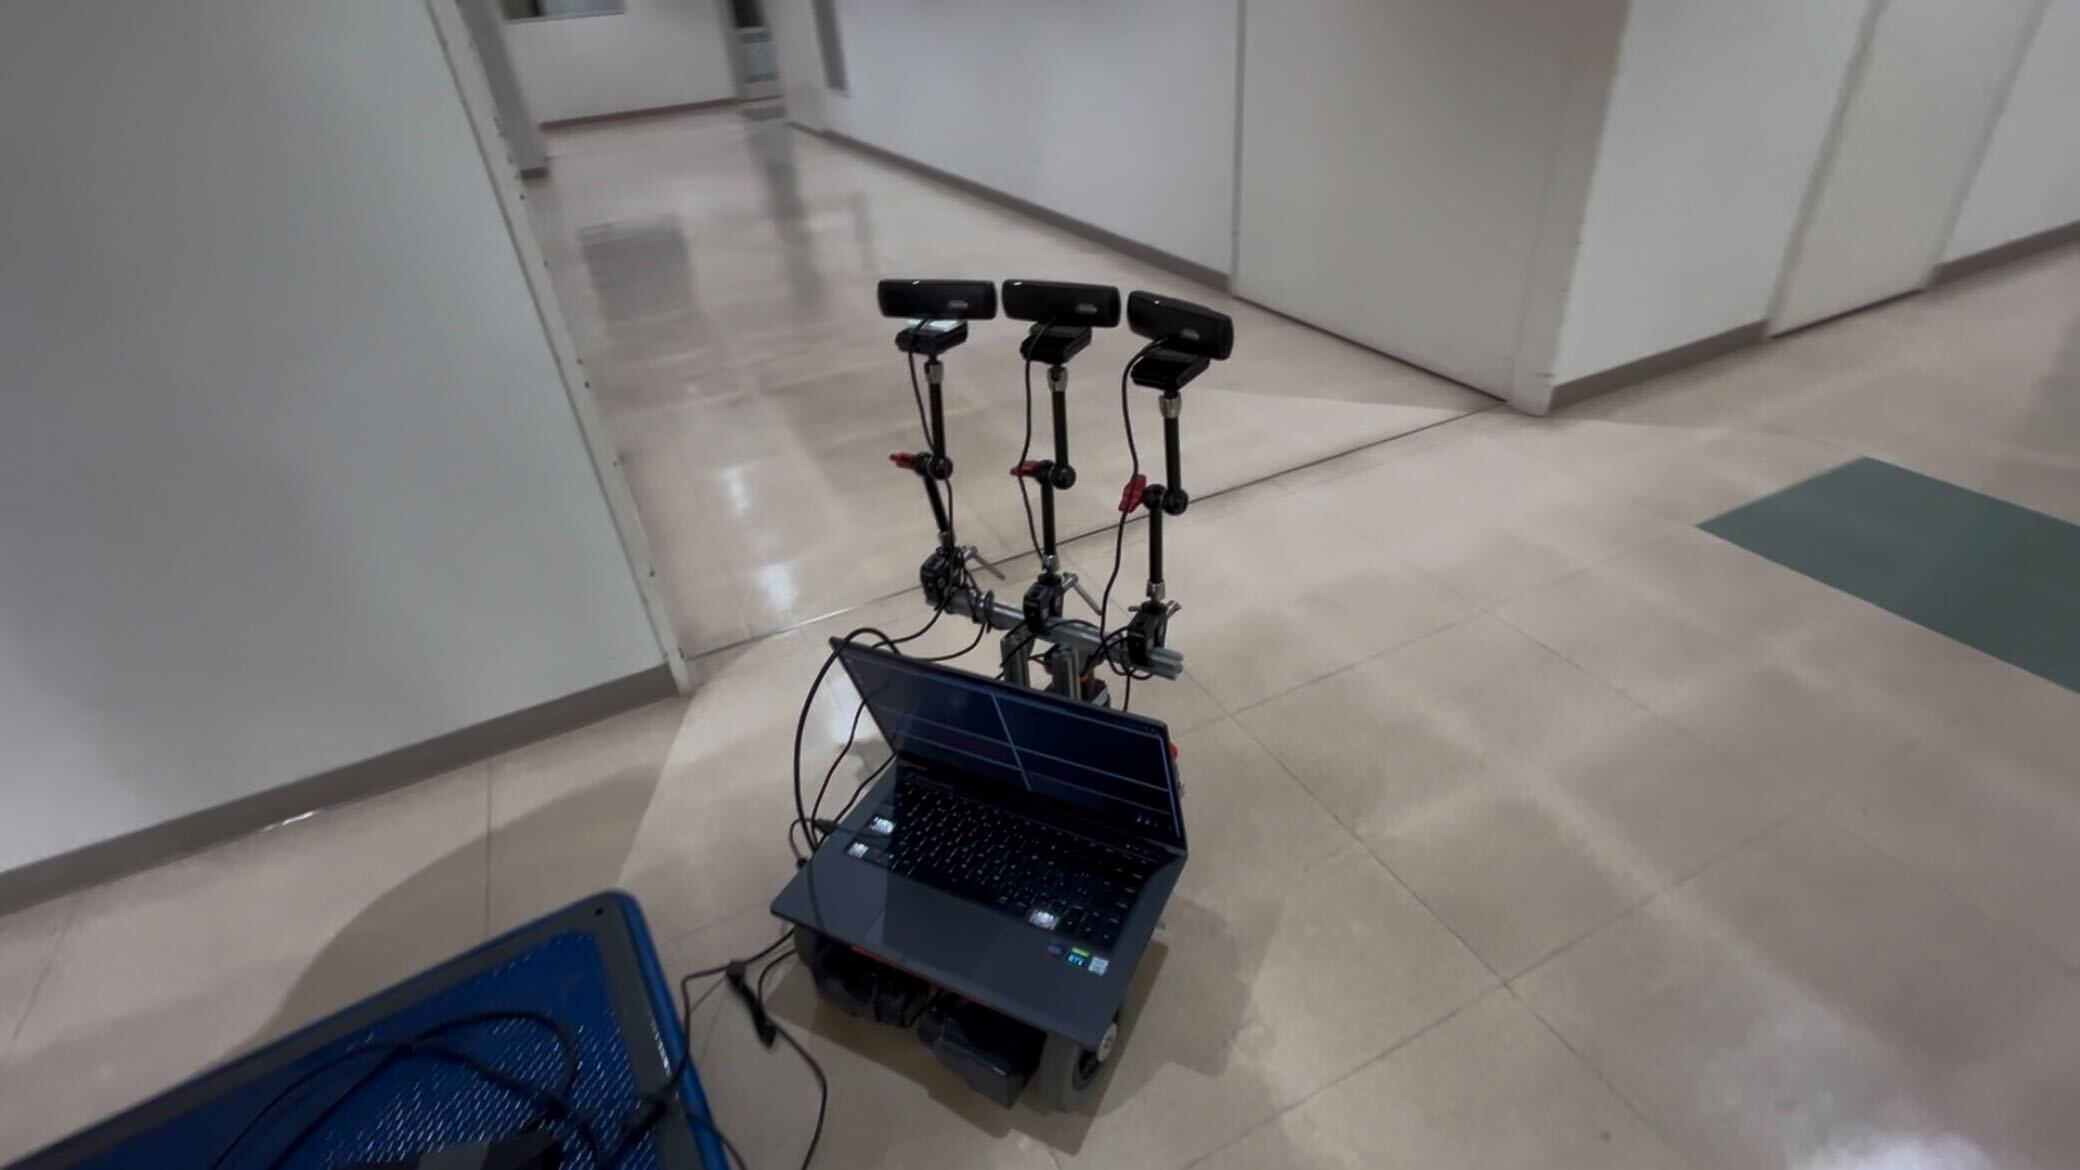
\includegraphics[keepaspectratio, width=55mm]{images/png/ishiguro/exp_7.png}
            \subcaption{左折}
        \end{minipage} \\
        \begin{minipage}[t]{0.5\textwidth}
            \centering
            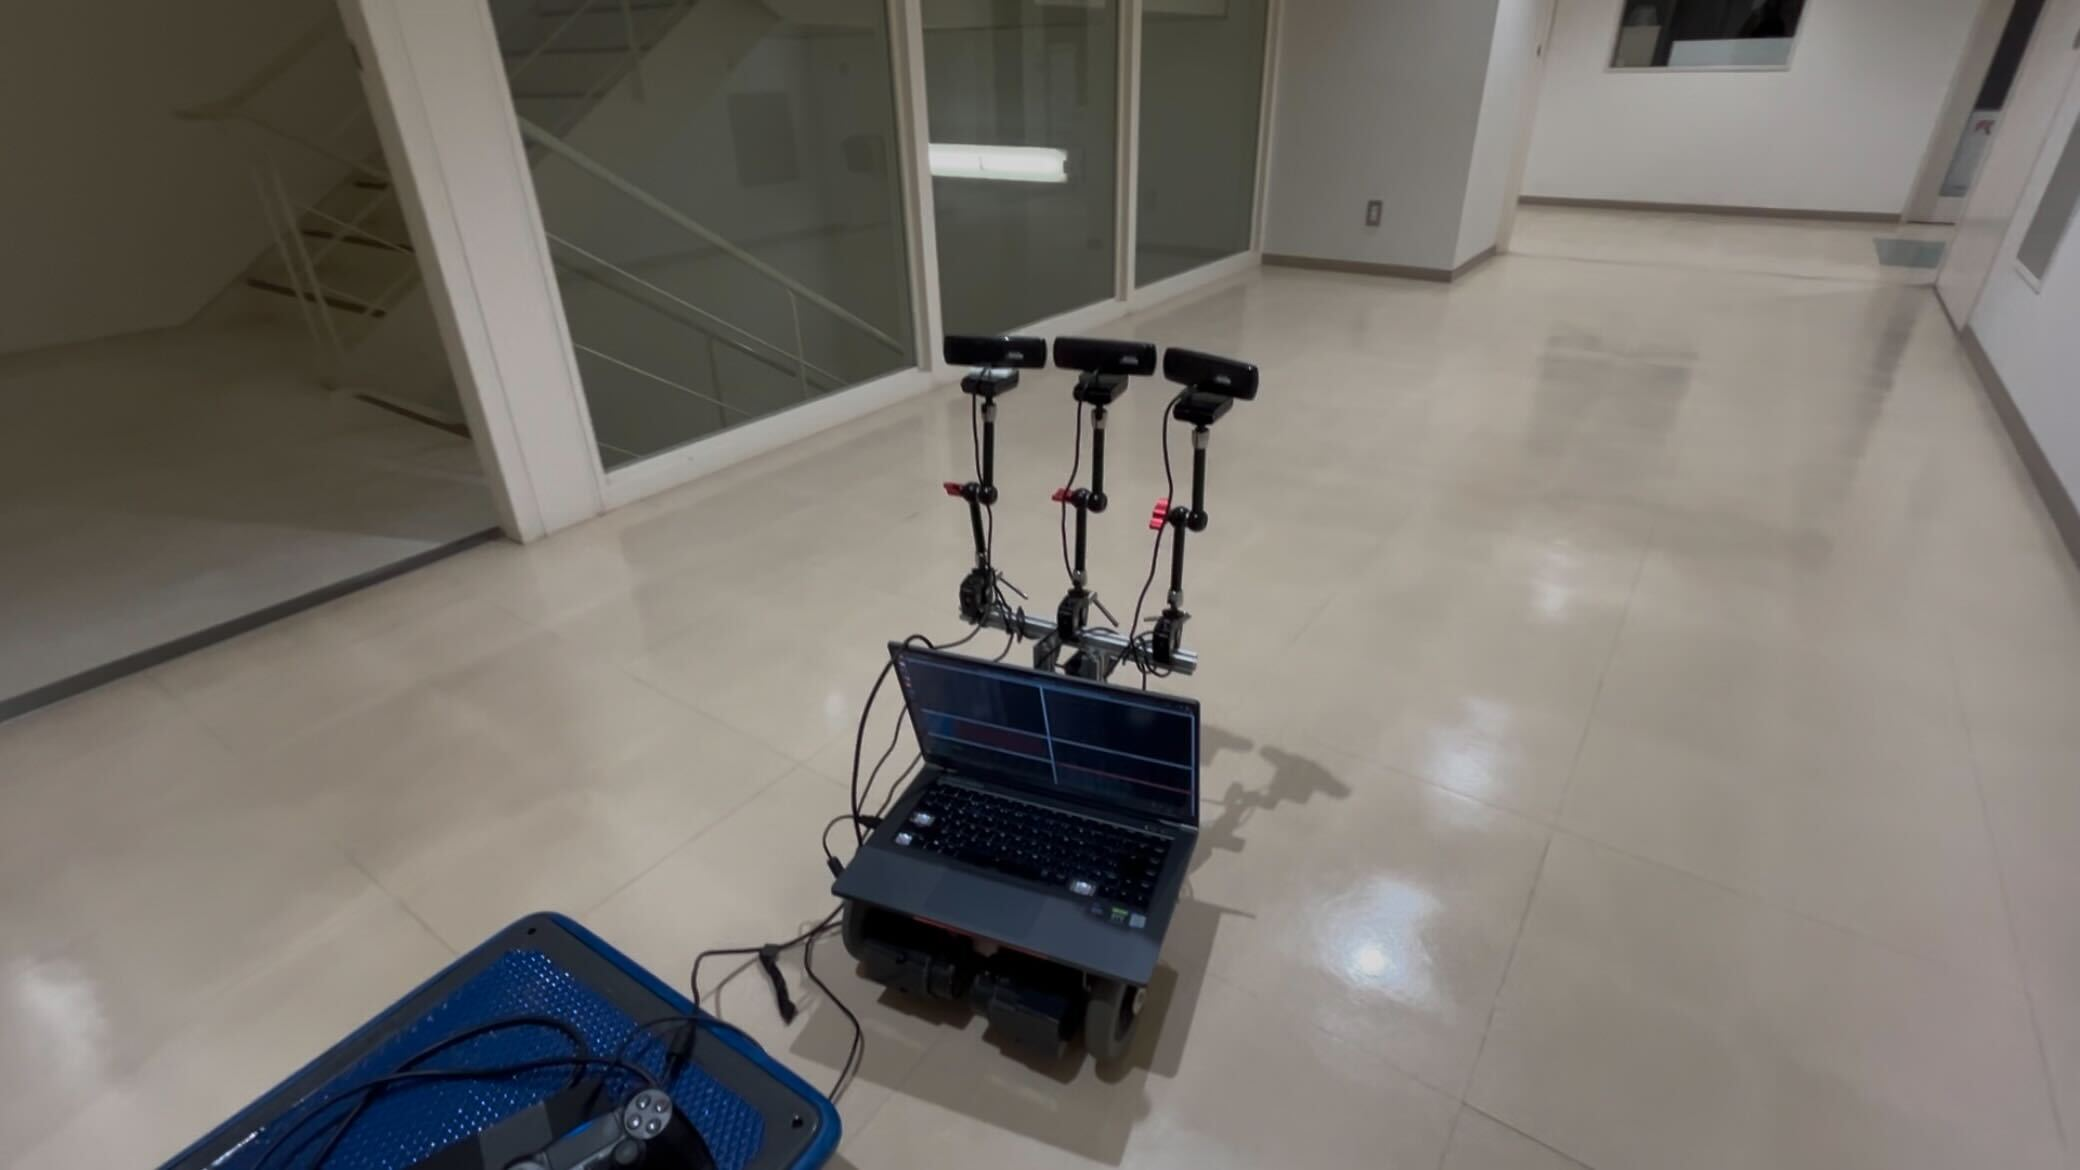
\includegraphics[keepaspectratio, width=55mm]{images/png/ishiguro/exp_8.png}
            \subcaption{突き当たりまで直進}
        \end{minipage} &
        \begin{minipage}[t]{0.5\textwidth}
            \centering
            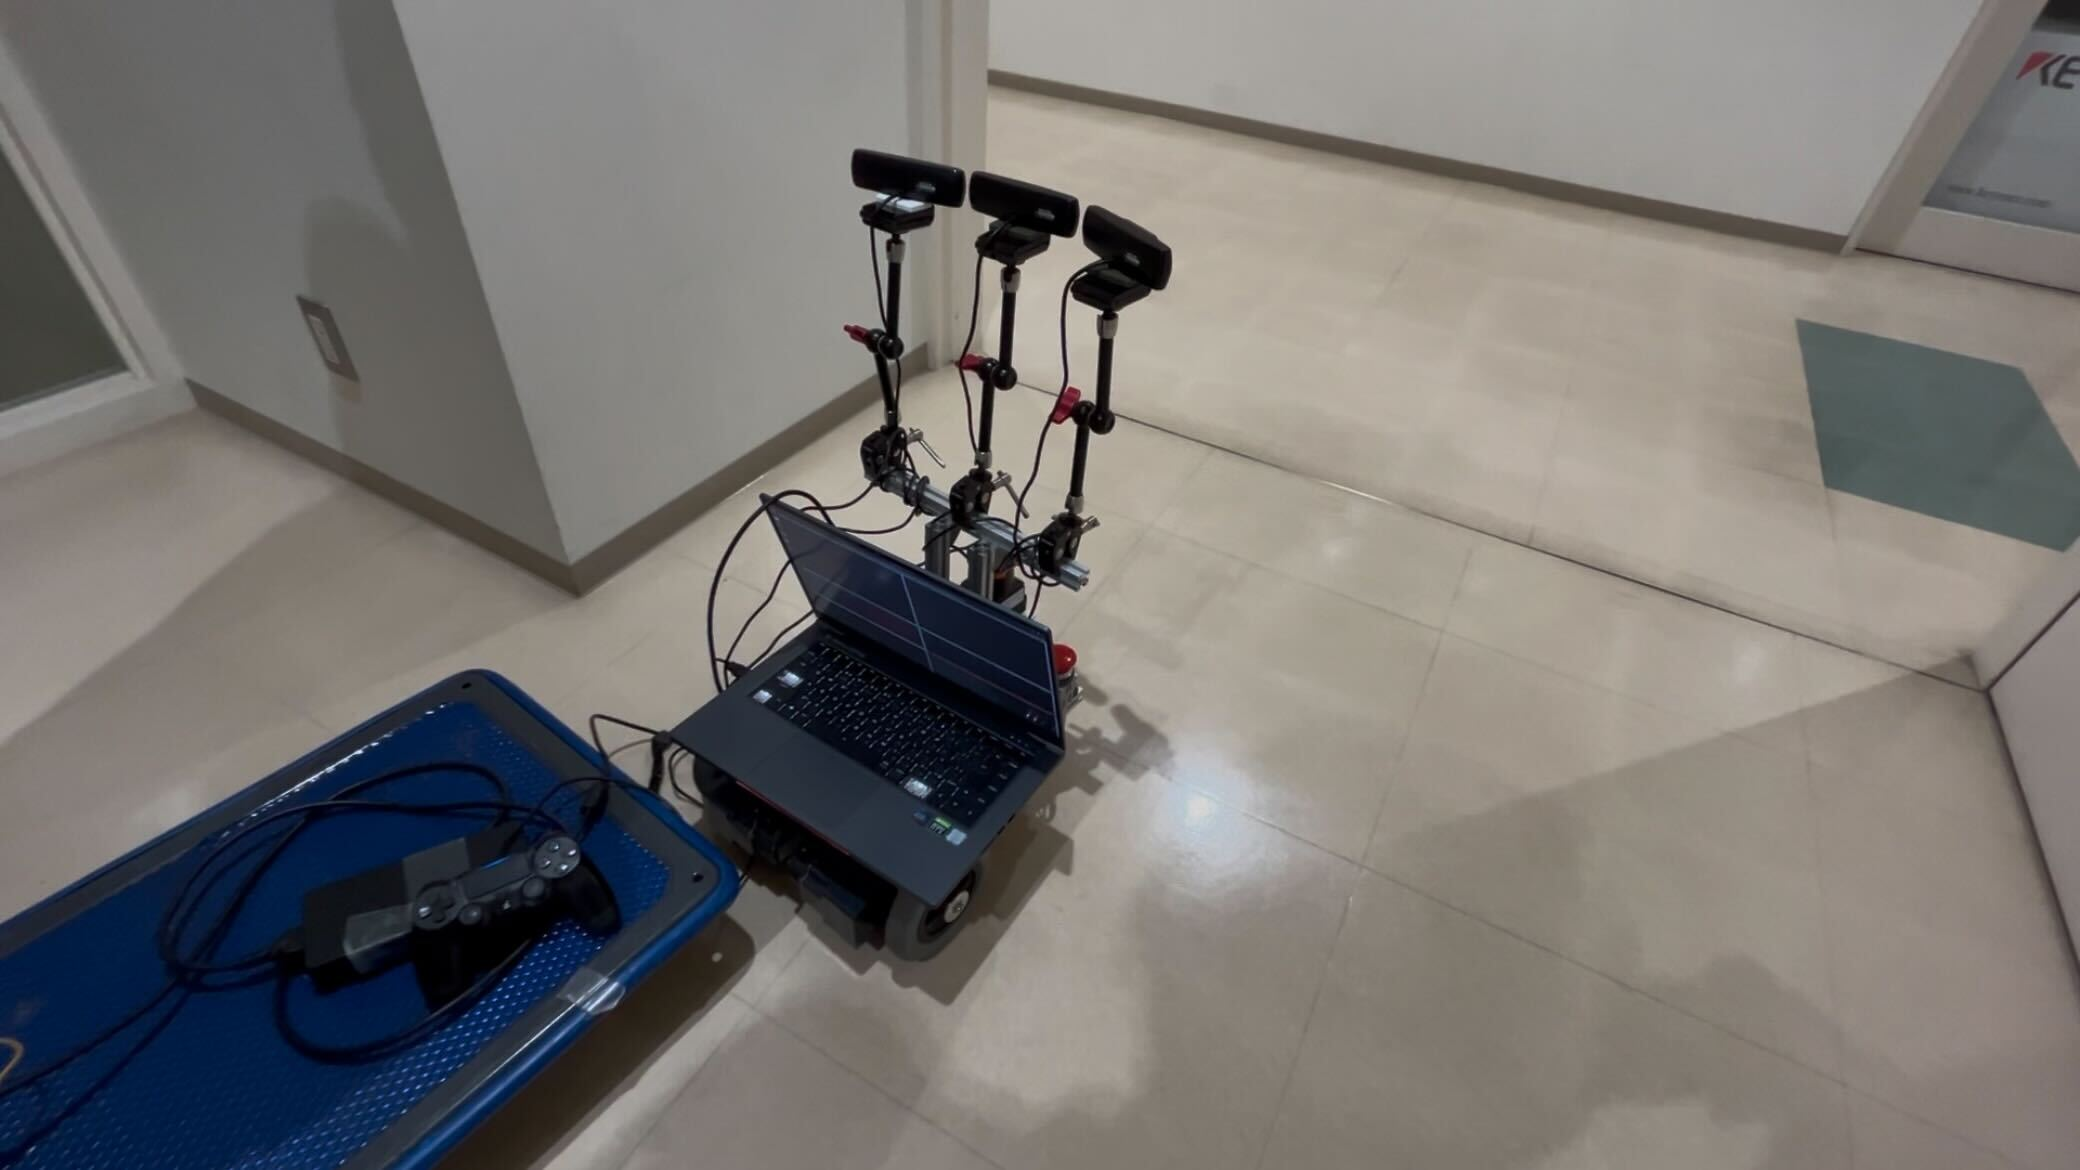
\includegraphics[keepaspectratio, width=55mm]{images/png/ishiguro/exp_9.png}
            \subcaption{停止}
        \end{minipage}
    \end{tabular}
\caption{An example of the robot applied the proposed system}
\label{fig:exp_path}
\end{figure*}

先行研究で走行が確認されていないエリアでも,ロボットがシナリオの道順に沿って,分岐路で適切な経路を選択する様子が確認できた.

失敗した4例ではそれぞれ,曲がり角で左折すべきところを直進した.
以下\figref{fig:miss}に失敗した箇所を示す.
失敗した4例の内訳として,\figref{fig:miss}の青枠に示す失敗が3例,緑枠に示す失敗が1例となった.
失敗した箇所でも通路の特徴の分類は正しく行われており,経路追従モジュールに与えられる目標方向も正しい値が入力されていた.
失敗の原因をとして,通路分類の結果の切り替わりが遅いことが考えられる.
以下に示す画像は学習時に「左折」の目標方向を与えたタイミングでのロボットの位置である.
〜〜に示す画像は,通路の分類が切り替わったタイミングで撮影したロボットの位置を表す.
このように分類遅れることで経路追従モジュールに目標方向が与えられるのが学習時より遅いことが確認できた.
確認として,学習時と同じタイミングで経路追従モジュールに目標方向を与えた場合,左折する様子が確認できた.
このことから,失敗要因として通路分類の切り替わりが遅いことが考えられる.

\begin{figure}[htbp]
    \centering
    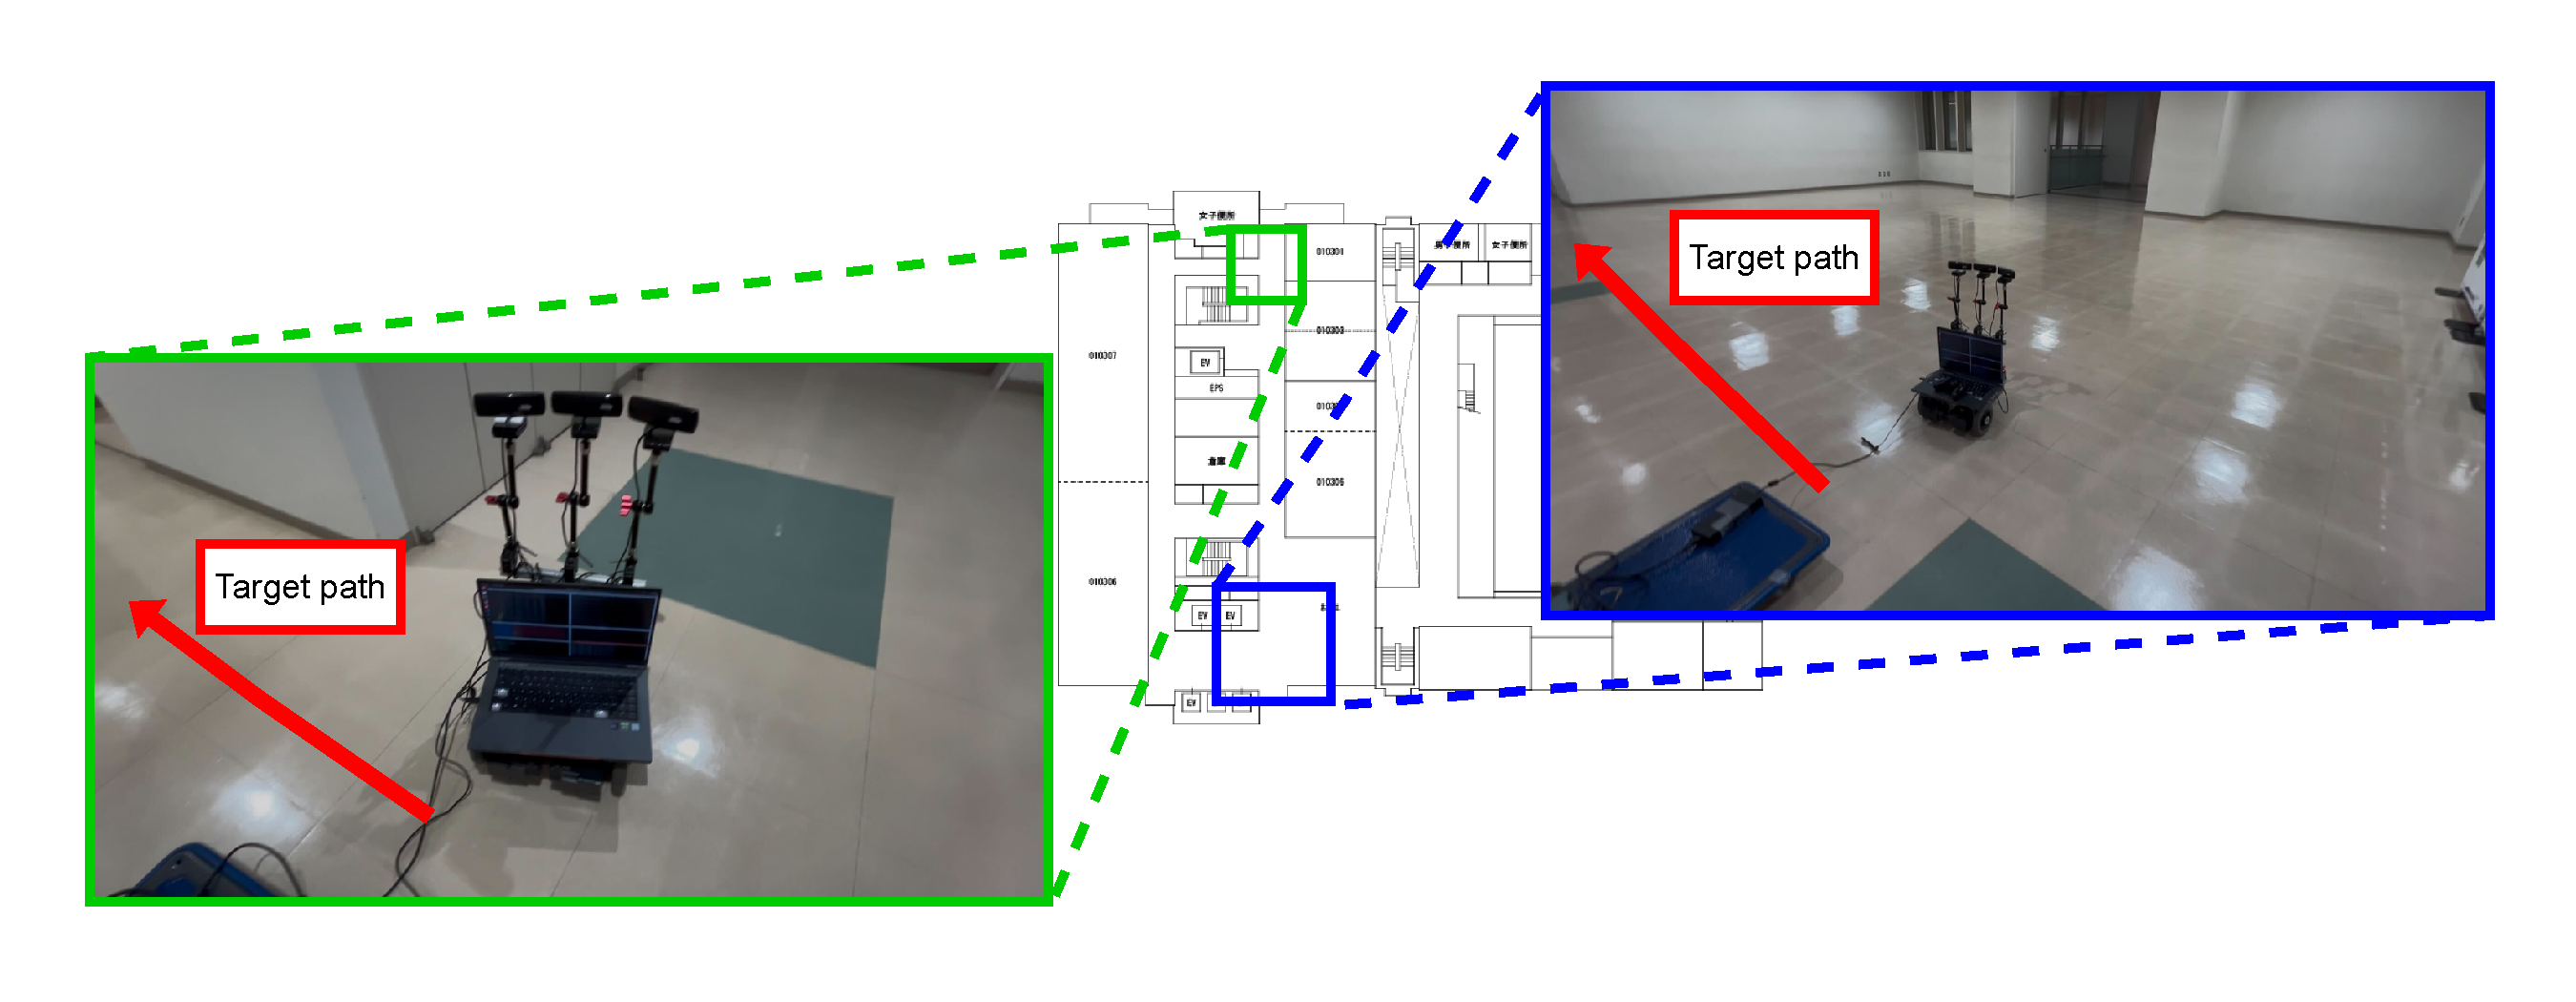
\includegraphics[width=130mm]{images/pdf/ishiguro/miss.pdf}
    \caption{Failed place}
    \label{fig:miss}
  \end{figure}